% {{{
\documentclass[12pt]{article}
\usepackage[tmargin=0.75in,bmargin=0.75in,lmargin=0.9in,rmargin=0.9in]{geometry}

\usepackage{amsmath}
\include{latexsym}
\include{amssymb}
\usepackage{enumitem}
\usepackage[symbol, hang]{footmisc}
\usepackage{indentfirst}
\usepackage{amssymb}
\usepackage{hyperref,graphicx,psfrag}

\def\F{\mathcal{F}}
\def\M{\mathcal{M}}
\def\dimspec{\mathfrak{D}}
\def\htop{h_{top}}
\def\trans{\mathcal{T}}
\def\G{\mathcal{G}}
\newcommand{\Z}{\mathbb{Z}}
\pagenumbering{gobble}
\def\O{\mathcal{O}}

\newcommand\NoIndent[1]{%
  \begingroup
  \par
  \parshape0
  #1\par
  \endgroup
}
%sets align environment spacing
\setlength{\jot}{3ex}
\DeclareMathOperator*{\argmax}{arg\,max}
\DeclareMathOperator*{\argmin}{arg\,min}

% Julia CodeBlock settings {{{
% \usepackage{listings}
\usepackage{color}
\usepackage[T1]{fontenc}
\usepackage{beramono}
\usepackage{listings}
	\usepackage[usenames,dvipsnames]{xcolor}

\lstdefinelanguage{Julia}%
  {morekeywords={abstract,break,case,catch,const,continue,do,else,elseif,%
      end,export,false,for,function,immutable,import,importall,if,in,%
      macro,module,otherwise,quote,return,switch,true,try,type,typealias,%
      using,while},%
   sensitive=true,%
   alsoother={$},%
   morecomment=[l]\#,%
   morecomment=[n]{\#=}{=\#},%
   morestring=[s]{"}{"},%
   morestring=[m]{'}{'},%
}[keywords,comments,strings]%

\lstset{%
	language         = Julia,
	basicstyle       = \ttfamily,
	keywordstyle     = \bfseries\color{cyan},
	stringstyle      = \color{magenta},
	commentstyle     = \color{ForestGreen},
	showstringspaces = false,
	breaklines	 =true,
	postbreak	 =\mbox{\textcolor{red}{$\hookrightarrow$}\space},
}
% }}}
\usepackage[english]{babel}
\usepackage{csquotes}

\usepackage[
backend=biber,
authordate-trad,
]{biblatex-chicago}

\addbibresource{citations.bib} %Imports bibliography file

\pagenumbering{arabic}
% }}}

% Title {{{
\begin{document}

\begin{titlepage}
   \begin{center}
       \vspace*{1cm}

       \textbf{INTERNAL AND EXTERNAL EFFECTS OF SOCIAL DISTANCING IN A PANDEMIC}

       \vspace{0.5cm}
        Examining a Socially Optimal Covid Policy \\ Reflecting Agent's Desire to Internalize their own Risk
            
       \vspace{1.5cm}

       \textbf{Ephraim Sutherland}

       \vfill
            
       % A projected presented for the completion of \\ Econ 475\\
            
       \vspace{0.8cm}

     
       % \includegraphics[width=0.4\textwidth]{covid19}
            
       Professor Tony Smith\\
       Econ 475\\
       \today
            
   \end{center}
\end{titlepage}

% }}}
\begin{center}
	{\large \bf The Social Planner}  
\end{center}

\setcounter{page}{2}

\section{Project}
 % project description {{{
\subsection{Description}
In this project, I will be implementing the model presented in the 2020 working paper by Farboodi, Jarosch, and Shimer \autocite{shimer}. In this paper, Shimer et al. explore the optimal activity path
of both individuals, and a social planner in a pandemic. Their work follows from the observation, according to cell phone location data, that at the start of the pandemic,
individuals on an aggregate level responded to the risk
of contracting Covid-19 resulting in an early drastic reduction in social activity irrespective of government lock down measures.
This observation is also supported by work in a recent paper by Goolsbee and Syverson, where, using SafeGraph data, they find that while social activity fell by 60 
percentage points, stay-at-home orders explain only 7 percent of that early reduction in activity \autocite{goolsbee}.

\subsection{Setup}
We begin with the standard epidemiological SIR model with the possibility of Death (SIRD) and then incorporate activity into our model.

\subsection{The Basic SIRD Model}
The SIRD model is a standard epidemiological compartmental model for the spread of a disease with the possibility of death. The model places every individual of a population into four different compartments:
Susceptible (S), Infected (I), Recovered (R), or Dead (D).

The ordering S,I,R,D also suggests the motion an individual may take through these compartments starting as
Susceptible, then becoming infected with some probability, and then recovering or dying based on the properties of the disease.

All four states always sum to the total population (which we can normalize to one) and transitions between the four is governed by a set of ODE's, a version of which is presented in (2) - (5). 
In these transition equations, Shimer et al. adapt the standard SIR model make the number of susceptible and infected individuals incorporate activity thereby endogenizing the effective transmission rate.

More specifically, we assume people do not know if they are infected or susceptible, but do know if they have recovered. Thus the rate at which susceptible individuals become infected is
$\beta A_s(t) N_s(t) A_i(t) N_i(t)$ where  $\beta > 0$ represents the ease of transmitting the disease and $A_s,N_s$ represent the activity level and number of individuals susceptible at time $t$ and
$A_i, N_i$ for those infected at time $t.$

\underline{\bf preferences over social activity}: By incorporating activity into the model Shimer et al. are able to look at how agents with a preference for activity respond to the 
risk of contracting the disease. Because increased activity also increases the spread and risk of contracting the disease, there is a constant trade off between the utility gained
from activity and the increased possibility of illness or even death. 

Shimer et al. approach this by assuming individuals have a preference for activity and get utility $u(a(t))$ from a level of social activity  $a(t) \geq 0$.
For simplicity, as in Shimer's paper, we 
assume agents have uniform preferences for activity denoted by the utility function $u(a) = log(a) - a + 1$ for an activity level $a.$ (Note, to allow for activity levels of zero, 
I actually use $u(a) = log(a+\varepsilon) - a + 1$ for some  small $\varepsilon > 0$).


\subsection{Socially Optimal Activity Path}
While Shimer et al. examine both a laissez-faire equilibrium and the socially optimal equilibrium, I will be focusing on the Socially optimal activity level.
For the social planning problem, the planner derives utility $u(A(t))$ for a given activity level weighted by the current fraction of the population infected 
or susceptible at time $t$. This reflects the idea that the social planner prefers activity or normal economic activity but has to weight this 
activity contingent on the current state of the pandemic, thus recognizing the externalities of activity.

We also assume that individuals, once recovered, are conferred with immunity and thus don't affect the change in susceptibility or number of individuals infected. The social planners problem is thus
to find the paths $A(t)$ and $A_r(t)$ which solve equation (1) subject to the growth dynamics dictated in equations (2) - (5).
In addition, we assume individuals discount the future at rate $\rho$ and that a cure is found at rate $\delta$. In light of our current vaccine which was 
found more quickly than anticipated, we could potentially view $\delta$ as the expected vaccination rate. $\rho$ and $\delta$ as well as the other parameters of the model are outlined in further detail in table \ref{table:parameters}.

\begin{align} 
	\max_{\{A(t), A_r(t)\}} \int_0^\infty 
	e^{-(\rho + \delta)t}
	&\left[
		(N_s(t) + N_i(t)) u(A(t)) + N_r(t) u(A_r(t)) - \gamma N_i(t) k
	\right]
	dt \\
	\text{subject to} \qquad N_s'(t) &= -\beta A(t)^2 N_s(t) N_i(t), \\
			N_i' (t) &= \beta A(t)^2 N_s(t) N_i(t) - \gamma N_i(t) \\
			N_r'(t) &= (1 - \pi) \gamma N_i(t) \\
			N_d'(t) &= \pi	\gamma N_i(t)
\end{align} 

To solve this, first, we can observe that $A_r(t)$ is not bound by constraints (2)-(5). This follows directly from our assumption that recovered individuals are immune.
So with utility function  $u(a) = log(a) - a + 1$, we can simply let $A_r(t) = 1$ thus maximizing $u(A_r(t)) = 0 \; \forall t $. 

Our planner's problem is then:

\begin{align}
	\max_{\{A(t) \}} \int_0^\infty 
	e^{-(\rho + \delta)t}
	&\bigg(
		[N_s(t) + N_i(t)] u(A(t)) - \gamma N_i(t) k
	\bigg)
	dt
\end{align} 

\subsection{Discretizing the Model}

Next, we begin by adapting our continuous time model to discrete time. Starting with our constraints, we can rewrite (2) - (5) as

\begin{align}
	N_s (t) &= N_s (t-1) -\beta A(t-1)^2 N_s(t-1) N_i(t-1), \\
	N_i (t) &= N_i (t-1)  + \beta A(t-1)^2 N_s(t-1) N_i(t-1) - \gamma N_i(t-1) \\
	N_r (t) &= N_r(t-1) + (1 - \pi) \gamma N_i(t -1) \\
	N_d(t) &= N_d(t-1) + \pi \gamma N_i(t-1)
\end{align} 

We can also rewrite (6) in discrete form as in equation (11). Note, I'm using $A(t)$ and $A_t$ interchangeably whenever one form feels more concise.
We also must change our continuous time discount factor to discrete time.
Let $\eta =  e^{-(\rho + \delta)} \approx 0.998029 $ represent our discrete time effective discount rate for the future. 
% \ref{table:parameters}.

% \int_0^1  e^{-(\rho + \delta)t} dt = \frac{1}{\rho + \delta} [1 - e^{-(\rho + \delta)} \approx 0.999014 

\begin{align}
	\max_{\{A_t\}} \sum_{t=0}^{\infty} \eta^t 
	\bigg( 
		[N_s(t) + N_i(t)] u(A_t) - \gamma N_i(t) k
	\bigg)
\end{align} 


We can also observe that $\eta < 1$ so it follows that we can solve (11) using our recursive formulation as in equation (12).

To solve (12), let our activity $A_t$ lie on a grid of $N$ points in the set $\bar{A} \equiv (A_1, A_2, A_3, \ldots, A_N)$ where $A_i \in [0,1]$
which we can rewrite in terms of recursive bellman equations.
\\
This reduces to finding $v(\cdot)$ such that

\begin{align}
	v(N_s, N_i) = &\max_{A \in \bar{A}} \bigg[ \big( [N_s + N_i] u(A) - \gamma N_i k \big) + \eta v(N_i', N_s') 
	\bigg]
\end{align}                         

where $X'$ marks the variable  $X$ in the next period.

Iterating on (12) until convergence, we constructed the value function as shown in figure \ref{fig:figure2}. In solving (12) we also construct our optimal decision rule $g : \{N_s\} \times \{N_i\} \to \bar{A}$.
where  

\begin{align}
	g(N_s, N_i) = \argmax_{A \in \bar{A}} \bigg[ \big( [N_s + N_i] u(A) - \gamma N_i k \big) + \eta v(N_i', N_s') \bigg] 
\end{align}

We can then use $g$ to construct our dynamic path for $\{A_t\}_{t=0}^{\infty}$ as well as $\{N_i(t), N_s(t), N_d(t), N_r, R(t)\}_{t=0}^{\infty}$ as shown in figure \ref{fig:figure1} where $R(t)$ is the effective 
reproduction number for the disease given by $R(t) = R_0 A(t)^2 N_s(t)$ where $R_0$ is the basic reproduction number $R_0 = \beta / \gamma$ 
-- the expected number of susceptible people infected by an infected person where almost everyone is susceptible and unaware of the disease.

The julia code describing equations (12) and (13) is outlined at the end of the paper (\ref{code:block1}) and included in its complete form in the second file submitted via canvas.

% }}}

In the rest of this paper I present the results of the simulations from different initial values and towards the end consider 
an optimal activity path given our current vaccination rate and exposure to Covid-19.

\newpage
\begin{center}
	\textbf{Simulation}\par\medskip
	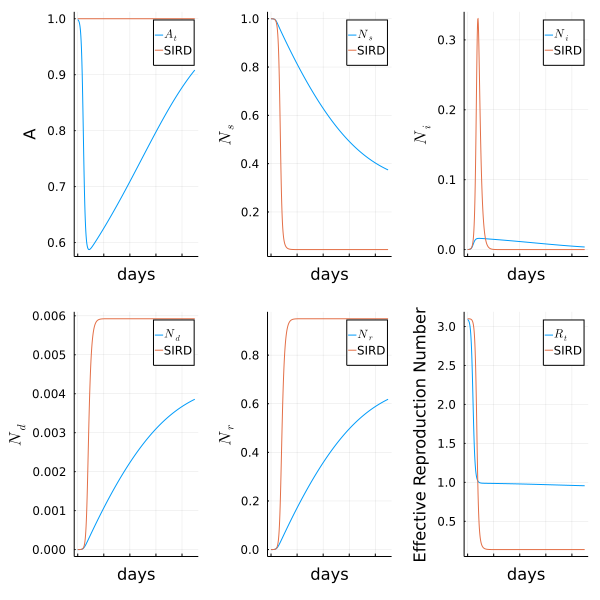
\includegraphics[width = \textwidth]{../plots/plots1.png}
	\text{Figure 1: {\bf Simulation for 450 days}}\par\medskip
	\label{fig:figure1}
\end{center}

Here \emph{SIRD} is the path predicted by the standard SIRD model which assumes activity is always 1, ie $A=1$.

In figure 1, we examine the dynamic paths for 450 days from the initial values of $N_s(0) = 0.9999223$ and $N_i(0) = 0.0000527$ as described in the parameters table \ref{table:parameters}.
We can see that the model states that, rather than attempting to push the reproduction immediately to zero, to push it slightly below 
one so that it effectively dies out without needing to completely stop all activity which is less aggressive then a complete lock down.

\begin{center}
	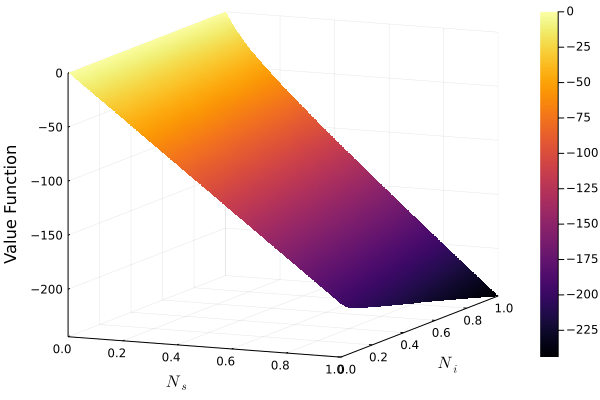
\includegraphics[width = \textwidth]{../plots/valueFunction_Surface.png}
	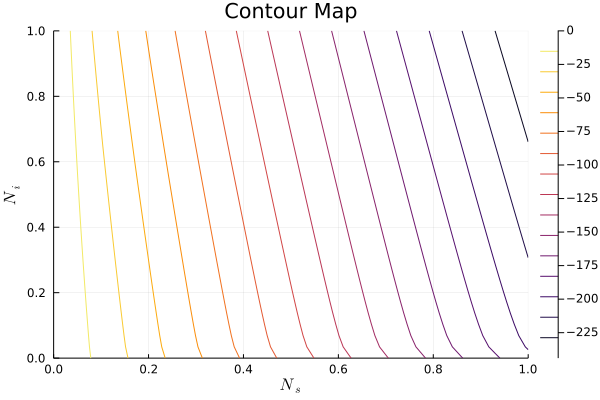
\includegraphics[width = \textwidth]{../plots/valueFunction_Contour.png}
	\text{Figure 1.5: {\bf Value Function}}\par\medskip
	\label{fig:figure2}
	% \textbf{Value Function}\par\medskip
\end{center}

\newpage

{\bf and decision rule, g.}

\begin{center}
	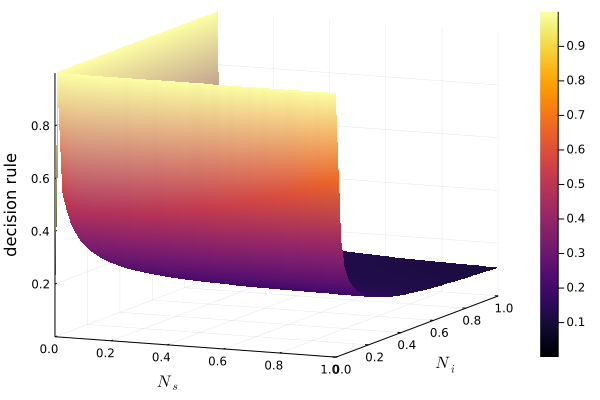
\includegraphics[width = \textwidth]{../plots/g_surface.png}
	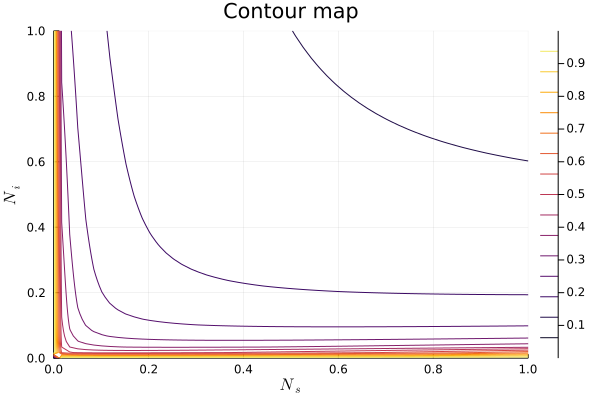
\includegraphics[width = \textwidth]{../plots/g_contour.png}
	\text{Figure 3: {\bf Decision Rule}}\par\medskip
\end{center}

We can clearly see from our contour map of $g$, that as either $N_i$ or $N_s$ go to zero, that our decision rule permits a higher $A$ approaching 1 as either $N_i$ or $N_s$ go to zero.
Note, when using a coarse grid, our decision rule permits a small anomaly around $g(0,0)$ but as our grid becomes finer, this hole disappears. This is likely due to my decision to use the utility function
$u(a) = log(a + \varepsilon) - a + 1$ where the epsilon begins to have a small effect for activity levels close to zero. However, it seems important to do this to allow for an activity level of zero 
representing total lock down (assuming this could be achieved).


Finally, we can consider initial scenario closer to today. Assuming a population of 320 million in the US and following the current trends of 31,000 positive cases per day, 
if we assume everyone who's received at least one does of the vaccine is fully immune, then we can assume initial starting values of $N_i(0) = 31000/320000000$, $N_r(0) = 0.47$ and  $N_s(0) = 1 - N_i - N_r(0)$.
Furthermore, if we assume 90\% of americans are vaccinnated within a year as our rate of a cure $\delta$, then we find a path like the one shown in figure 4, below. We can immediately observe that the optimal
activity level stays quite high hardly dipping below 0.85. The model also assumes we are starting at full activity which is not the case so spread will likely be far less than predicted in the graphs in 
figure 4. However, we can already observe that the actual number of individuals infected still remains quite low hardly rising above 0 and then once again approaching zero as the simulated path develops. 
Also of note is the fact that our effective transmission rate starts quite low and we rapidly fall to below 1 ones again leading to the disease naturally dying out.

\begin{center}
	\textbf{Simulation for 450 days}\par\medskip
	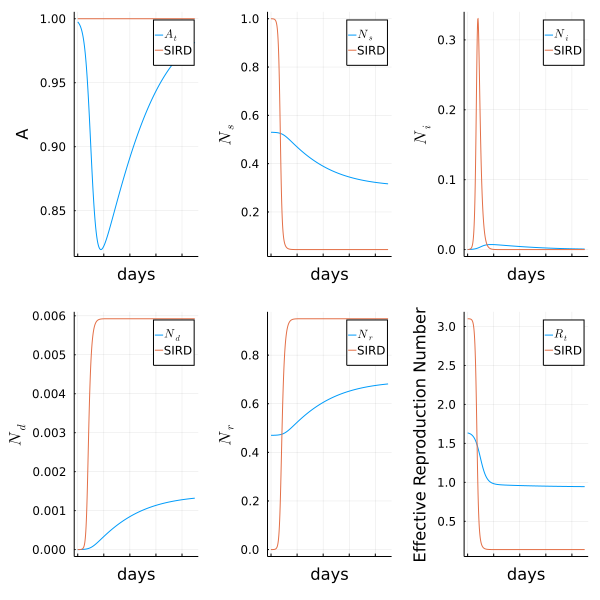
\includegraphics[width = \textwidth]{../plots/plots2.png}
	\text{Figure 4: {\bf Simulation for 450 days}}\par\medskip
	\label{fig:figure1_2}
\end{center}

The rest of this article summarizes the parameters used as well as the basic implementation of the bellman equations. The actual code is also included in a separate file submitted through canvas.


%Tables {{{
\newpage
{\bf \underline{Parameters:}}
\begin{table}[h!]
	\centering
	\begin{tabular}{||c c c c||} 
		\hline
		Parameter Descriptions 		& Parameters & Value & Target \\ [0.5ex] 
		\hline\hline
		Conditional transmission prob. 		& $\beta$ 	& $0.3 + \gamma$& Initial doubling time \\ 
		Rate that infectiousness ends 		& $\gamma$ 	& 1/7 		& Duration until symptomatic \\
		Infection fatality rate (IFR) 		& $\pi$ 	& 0.0062 	& Hall, Jones and Klenow (2020) \\
		Value of a statistical life (VSL) 	& $\nu$ 	& 31,755	& Hall, Jones and Klenow (2020) \\
		Arrival rate of cure 			& $\delta$ 	& 0.67/365 	& Exp. time until vaccine/cure \\
		Discounting 				& $\rho$ 	& 0.05/365	& Annual discount rate \\
		Fraction initially affected 		& $N_i(0)$ 	& 0.0000527 	& Deaths before March 13, 2020 \\ [1ex] 
		% \hline
	% \end{tabular}
% \end{table}

% \begin{table}[h!]
	% \centering
	% \begin{tabular}{||c c c c||} 
		\hline \hline
		Other & & & \\ [0.5ex] 
		\hline\hline
		Basic reproduction number 		& $R_0$ 	& $3.1$ & Implied by $\gamma$ and $\beta$ \\ 
		Expected cost of infection 		& $k$ 	& 197 		& Implied by $\pi$ and $\nu$ \\
		Fraction initially susceptible 		& $N_s(0)$ 	& 0.9999223 	& no social distancing before $t=0$ \\
		Discrete time discount rate 		& $\eta$ 	& 0.999014 	& $e^{-(\rho + \delta)}$ \\  %\int_0^1  e^{-(\rho + \delta)t} dt
		Effective Reproduction Number 		& $R_0*A(t)^2*(N_s(t))$ 	&  	& \\[1ex]
		\hline
	\end{tabular}
	\caption{Table to test captions and labels}
	\label{table:parameters}
\end{table}
% }}}

% Code Block {{{
\begin{lstlisting}


# returns (discrete) value and policy functions
function valueFuncIter(A; N = length(A), toler=1e-6, maxiter=1000, verbose=1, params=p)

	v0=zeros(N, N)
	g = fill(0.0, N, N) 
	grid1 = grid(0, 1, N)
	S = creategrid(0, 1, N); I = creategrid(0,1,N);

	err = 1+toler; niter = 0;
	tol = zeps = 1.0e-8

	while err > toler && niter < maxiter
		niter += 1
		v1 = copy(v0)

		interp_cubic = CubicSplineInterpolation((grid1, grid1), v0, extrapolation_bc=Line())

		# define new value function by iterating over all grid points
		for i in 1:N
			for j in 1:N
				fmin,xmin,niter = brent(0, 1/2, 1, a_j -> (-1*bellman(a_j, S[i], I[j], interp_cubic)), tol, zeps)
				v1[i, j] = -1*fmin
				g[i, j] = xmin
			end
		end
		err = maximum(abs.(v1 - v0)) # error defined using the sup norm
		v0 = v1
	end

	if err <= toler && verbose >= 1
		println("Value function iteration converged in $niter iterations (maxerr = $err)")
	elseif err > toler
		println("Value function iteration failed to converge in $niter iterations (maxerr = $err)")
	end
	return v0, g
end

function evolution(S, I, a; params=p )
	@unpack rho, pi, gamma, nu, delta, beta, k, eta= params
	S_new =S - beta*(a^2)*S*I
	I_new =I + beta*(a^2)*S*I - gamma*I
	return S_new, I_new
end

function bellman(a, S, I, spline; params=p)
	@unpack rho, pi, gamma, nu, delta, beta, k, eta= params
	S_prime, I_prime = evolution(S, I, a)
	return ((S + I)*U(a) - gamma*I*k) + eta*spline(S_prime, I_prime)
end
\end{lstlisting}
\label{code:block1}
% }}}

\newpage

\printbibliography
\end{document}

